\documentclass[tikz,border=8pt]{standalone}
\usetikzlibrary{arrows.meta,positioning,shapes.geometric}
\begin{document}
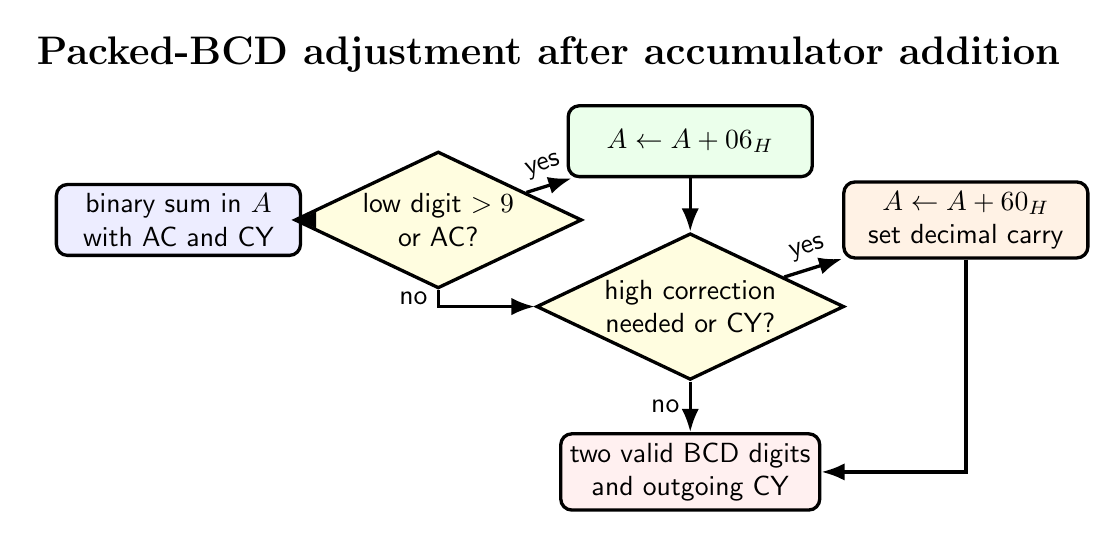
\begin{tikzpicture}[font=\sffamily,>=Latex,
 box/.style={draw,very thick,rounded corners,minimum width=3.1cm,minimum height=.9cm,align=center},
 test/.style={draw,very thick,diamond,aspect=2.1,align=center,inner sep=1.5pt}]
\node[font=\Large\bfseries] at (6.4,6.35) {Packed-BCD adjustment after accumulator addition};
\node[box,fill=blue!7] (sum) at (1.7,4.25) {binary sum in $A$\\with AC and CY};
\node[test,fill=yellow!12] (low) at (5.0,4.25) {low digit $>9$\\or AC?};
\node[box,fill=green!8] (six) at (8.2,5.25) {$A\leftarrow A+06_H$};
\node[test,fill=yellow!12] (high) at (8.2,3.15) {high correction\\needed or CY?};
\node[box,fill=orange!10] (sixty) at (11.7,4.25) {$A\leftarrow A+60_H$\\set decimal carry};
\node[box,fill=red!6] (done) at (8.2,1.05) {two valid BCD digits\\and outgoing CY};
\draw[very thick,->] (sum)--(low);
\draw[very thick,->] (low)-- node[above,sloped] {yes} (six);
\draw[very thick,->] (six)--(high);
\draw[very thick,->] (low.south) |- node[pos=.25,left] {no} (high.west);
\draw[very thick,->] (high)-- node[above,sloped] {yes} (sixty);
\draw[very thick,->] (sixty.south) |- (done.east);
\draw[very thick,->] (high)-- node[left] {no} (done);
\end{tikzpicture}
\end{document}
